%!TEX root = main.tex
\section{Warm-up: full-disclosure paths}

We first consider a disclosure policy that reveals the full history in each round $t$, \ie $m_t=\SubH{t-1}$; we call it the \emph{full-disclosure policy}. The info-path for this policy is a simple path. We use this policy as a ``gadget" in our constructions. Hence, we formulate it slightly more generally:
  
\begin{definition}
A subset of rounds $S\subset [T]$ is called a \emph{full-disclosure path} in the  info-graph $G$ if the induced subgraph $G_S$ is a simple path, and it connects to the rest of the graph only through the terminal node $\max(S)$, if at all.
\end{definition}
  
We prove that for a constant number of arms, with constant probability, a full-disclosure path of constant length suffices to sample each arm at least once. We will build on this fact throughout.

\begin{lemma}\label{lem:greedy}
There exist numbers $\fdpL>0$ and $\fdpP>0$ that depend only on $K$, the number of arms, with the following property. Consider an arbitrary disclosure policy, and let $S\subset [T]$ be a full-disclosure path in its info-graph, of length $|S|\geq \fdpL$. Under Assumption \ref{ass:embehave}, with probability at least $\fdpP$, subhistory $\SubH{S}$ contains at least once sample of each arm $a$.
\end{lemma}

\begin{proof}[Proof Sketch]
\ascomment{Jieming, pls add a brief proof sketch if you can.}
\end{proof}


We provide a simple disclosure policy based on full-disclosure paths. The policy follows the ``explore-then-exploit'' paradigm. The ``exploration phase" comprises the first $N = T_1\cdot \fdpL$ rounds, and consists of $T_1$ full-disclosure paths of length $\fdpL$ each, where $T_1$ is a parameter. In the ``exploitation phase", each agent $t>N$ receives the full subhistory from exploration, \ie $m_t = \SubH{[N]}$. The info-graph for this disclosure policy is shown in Figure~\ref{fig:2level}.

\begin{figure}[H]
\centering
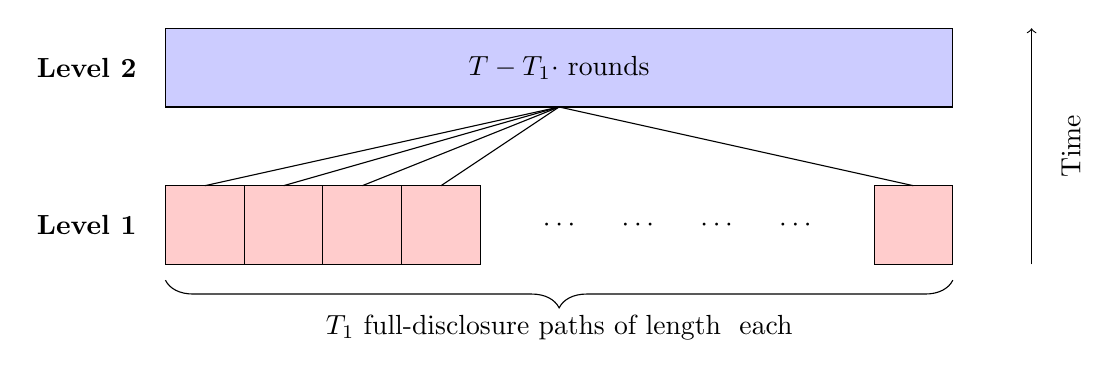
\begin{tikzpicture}
 \filldraw[fill=blue!20!white]
 (0,2)--(10,2)--(10,3)--(0,3)--cycle;
  \filldraw[fill=red!20!white]
  (0,0)--(1,0)--(1,1)--(0,1)--cycle;
  \draw (0.5,1)--(5,2);
  \filldraw[fill=red!20!white]
  (1,0)--(2,0)--(2,1)--(1,1)--cycle;
  \draw (1.5,1)--(5,2);
  \filldraw[fill=red!20!white]
  (2,0)--(3,0)--(3,1)--(2,1)--cycle;
  \draw(2.5,1)--(5,2);
  \filldraw[fill=red!20!white]
  (3,0)--(4,0)--(4,1)--(3,1)--cycle;
  \draw(3.5,1)--(5,2);
  \filldraw[fill=red!20!white]
  (9,0)--(10,0)--(10,1)--(9,1)--cycle;
  \draw(9.5,1)--(5,2);
  \node at(5,0.5){$\cdots$};
  \node at(6,0.5){$\cdots$};
  \node at(7,0.5){$\cdots$};
  \node at(8,0.5){$\cdots$};
  \node at(5,2.5){$T -T_1 \cdot \fdpL$ rounds};
  \node at(0.5,0.5){$\fdpL$};
  \node at(1.5,0.5){$\fdpL$};
  \node at(2.5,0.5){$\fdpL$};
  \node at(3.5,0.5){$\fdpL$};
  \node at(9.5,0.5){$\fdpL$};
  \node at(-1,0.5){\textbf{Level 1}};
  \node at(-1,2.5){\textbf{Level 2}};
  \draw[->] (11,0)--(11,3);
  \node at(11.5,1.5)[ rotate=90]{Time};

  \draw [decorate,decoration={brace,amplitude=10pt},xshift=0pt,yshift=0pt] (10,-0.2) -- (0,-0.2) node [black,midway,yshift=-0.6cm] 
  {$T_1$ full-disclosure paths of length $\fdpL$ each};
\end{tikzpicture}

\caption{Info-graph for the 2-level policy. }
%Each red box in level 1 corresponds to a path connecting a set of
%  $T_G$ agents. The entire history in level 1 is then aggregated and
%  shown to each agent in level 2.}
\label{fig:2level}
\end{figure}


It is useful to think of the info-graph as having two levels (corresponding to exploration and exploitation). Accordingly, we call this policy the \emph{\2LEVEL}. We show that it incentivizes the agents to perform non-adaptive exploration, and achieves a regret rate of  $\tilde O_K(T^{2/3})$. The key idea is that using many full-disclosure paths ``in parallel" ensures that sufficiently many samples of each arm are collected during exploration.

\begin{theorem}\label{thm:2level}
The \2LEVEL with parameter $T_1 = T^{2/3}\,\log(T)^{1/3}$ achieves regret
\[ \reg(T) \leq O_K\left( T^{2/3}\, \log(T)^{1/3} \right).\]
\end{theorem}

\begin{remark}
For a constant $K$, the number of arms, we match the optimal regret rate for non-adaptive multi-armed bandit algorithms. If the gap parameter $\Delta$ is known to the principal, then (for an appropriate tuning of parameter $T_1$) we can achieve regret 
  $\reg(T) \leq O_K(\log(T) \cdot \Delta^{-2})$.
\end{remark}

To simplify presentation of the proofs, we will make the following assumption.%
\footnote{This assumption can be removed, without any conceptual difficulty, but at the cost of a somewhat lengthier proofs.}
 

\begin{assumption}\label{ass:simplifying}
In each round $t$, the estimates $\hat{\mu}_{t,a}$ depend only the multiset 
    $\left\{\; (a_s,r_s):\;s\in S_t \;\right\}$,
called \emph{anonymized subhistory}. Each agent forms its estimates according to the same \emph{estimate function}: a function $f$ from subhistories to $[0,1]^K$, so that the estimate vector
        $(\hat{\mu}_{t,a}:\, a\in\A)$
equals $f(m_t)$. 
\end{assumption}

Among other things, this assumption allows us to the define the expected number of samples of a given arm $a$ collected by a full-disclosure path $S$ of length $\fdpL$ (\ie present in the subhistory $\SubH{S}$. Indeed, this number, denoted $\fdpN$, is the same for all such paths. Then,

\begin{lemma}\label{lem:t1runs}
Suppose the info-graph contains $T_1$ full-disclosure paths of $\fdpL$ rounds each. Let $N_a$ be the number of samples of arm $a$ collected by all paths. Then with probability at
  least $1-\delta$, for all $a\in \A$,
  \[
    \left| N_a - \fdpN T_1\right| \leq \fdpL\cdot \sqrt{T_1 \log(2K/\delta) / 2}.
  \]
\end{lemma}






%%% Local Variables:
%%% mode: latex
%%% TeX-master: "main"
%%% End:
